\documentclass[amsmath,amssymb, aps, prx, longbibliography, twocolumn]{revtex4-1}

\usepackage{natbib}
\usepackage{graphicx}% Include figure files
\usepackage{dcolumn}% Align table columns on decimal point
\usepackage{bm}
\usepackage[usenames]{color}
\usepackage{subfigure}

\newcommand{\cb}[1]{\textcolor{magenta}{[Carsten: #1]}}


\begin{document}

\title{ Detecting non-Fermi liquid transport in the quantum critical region \\ via quantum loop topography}

\author{George (Trey) Driskell$^1$}
\author{Samuel Lederer$^1$}
\author{Carsten Bauer$^2$}
\author{Simon Trebst$^2$}
\author{Eun-Ah Kim$^1$}
\email{eun-ah.kim@cornell.edu}

\affiliation{%
$^{1}$Department of Physics, Cornell University, Ithaca, New York 14853, USA}%
\affiliation{$^{2}$Institute for Theoretical Physics, University of Cologne, 50937 Cologne, Germany}

\date{\today}

\begin{abstract}
Anomalous transport, such as T-linear resistivity (a hallmark of non-Fermi liquid behavior), is a ubiquitous feature of strongly correlated metallic systems, but famously difficult to understand theoretically. For relevant simple models, the transport computations of even numerically exact Monte Carlo simulations are subject to enormous systematic errors and come at great additional computational cost. Building on earlier work, we apply quantum loop topography (QLT) and supervised learning on quantum Monte Carlo data to examine the Fermi liquid to non-Fermi liquid crossover in models of both Ising nematic and \cb{antiferromagnetic} spin density wave quantum criticality. Previous work on these models has demonstrated this crossover using measurements of correlation functions at nonzero imaginary time separation. Our results, using only equal time measurements, show good agreement with these previous results at dramatically lower computational cost. Hence, QLT-based machine learning can accelerate the exploration of parameter space in search for non-Fermi liquid behavior by obviating the need for expensive dynamical measurements.
\end{abstract}

\maketitle

%%%%%%%%%%%%%%%%%%%%%%%%%%%%%%%%%%%%%%%%%%%%%%%%%%%%%%%%%%%%%%%%%%
% Introduction
%%%%%%%%%%%%%%%%%%%%%%%%%%%%%%%%%%%%%%%%%%%%%%%%%%%%%%%%%%%%%%%%%%
[1 problem statement: NFL in QC -- Simon ]
Most often defined by transport in experiment, ubiquitous
\\
\\
\\
\\
\\
\\
\\
\\
\\
\\
\\


[2 literature in sign-free MC -- Simon]
Transport is hard. "proxies" are not satisfactory.
\\
\\
\\
\\
\\
\\
\\
\\
\\
\\
\\
\\
\\
\\
\\

[3 literature in phase recognition -- EK]
Ideal application of ML is where conventional approaches are lacking: such as topological order and NFL.
 \\
 \\
 \\
 \\
 \\
 \\
 \\
 \\
 \\
 \\
 \\
 \\
 \begin{figure} [t]
    \centering
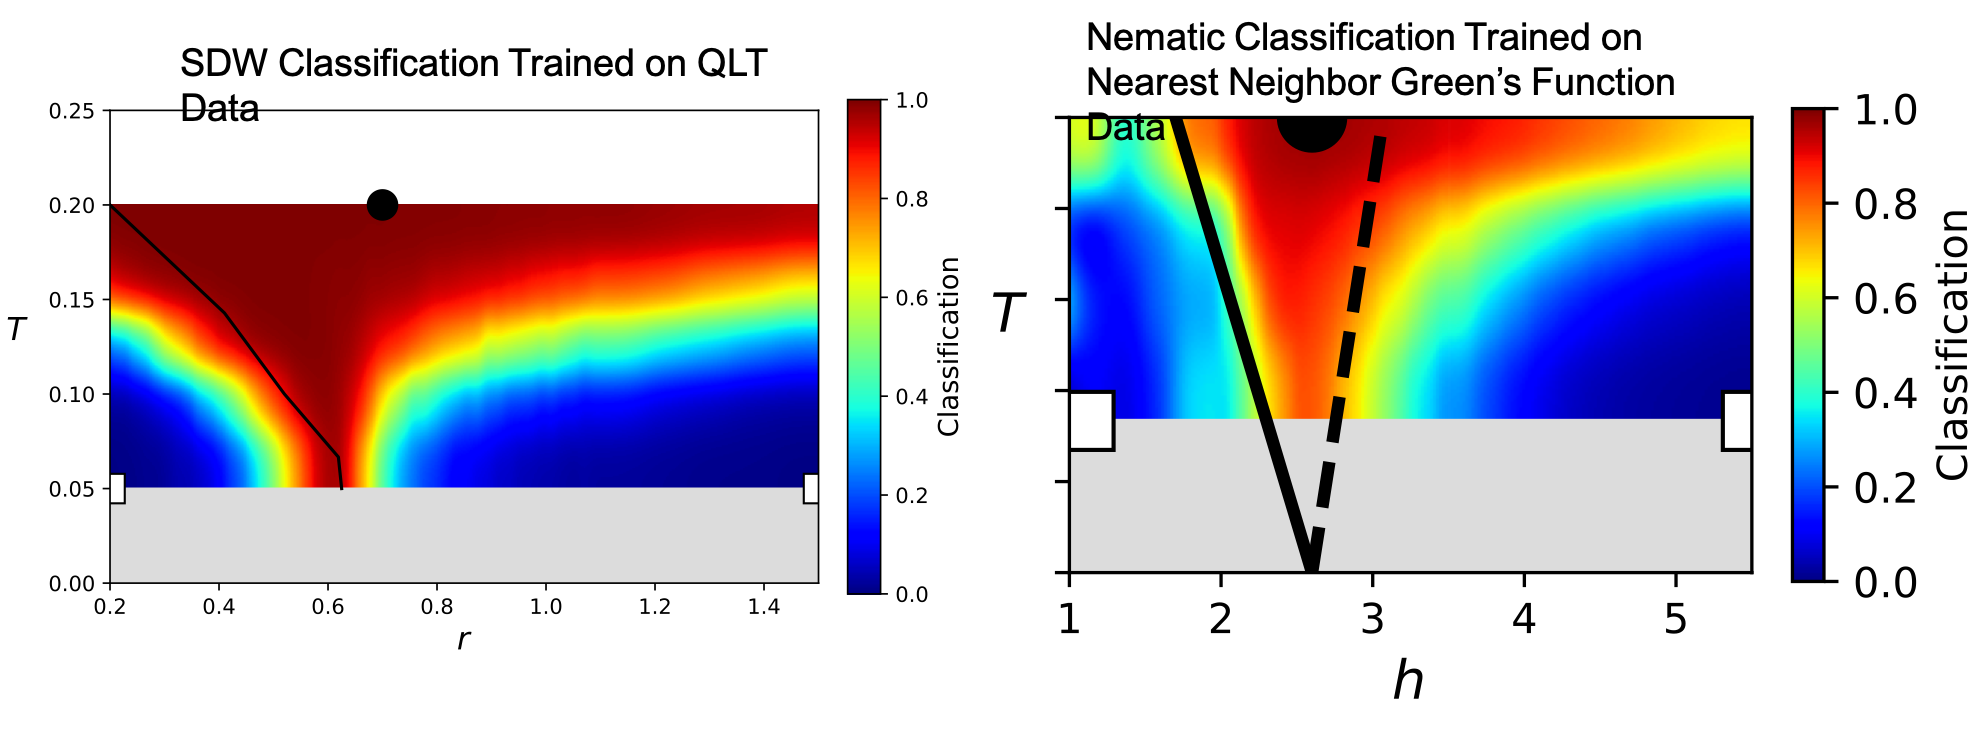
\includegraphics[width=.5\textwidth]{3PT-PDs.png}
    \caption{Caption}
    \label{fig:pds}
\end{figure}
[4 In this paper - Fig 1] 
\\
\\
\\
\\
\\
\\
\\
\\


[5 Two QCP's to study -- Sam]
Their similarities and differences in words.
\\
\\
\\
\\
\\
\\
\\
\\
\\

 \begin{figure} [t]
    \centering
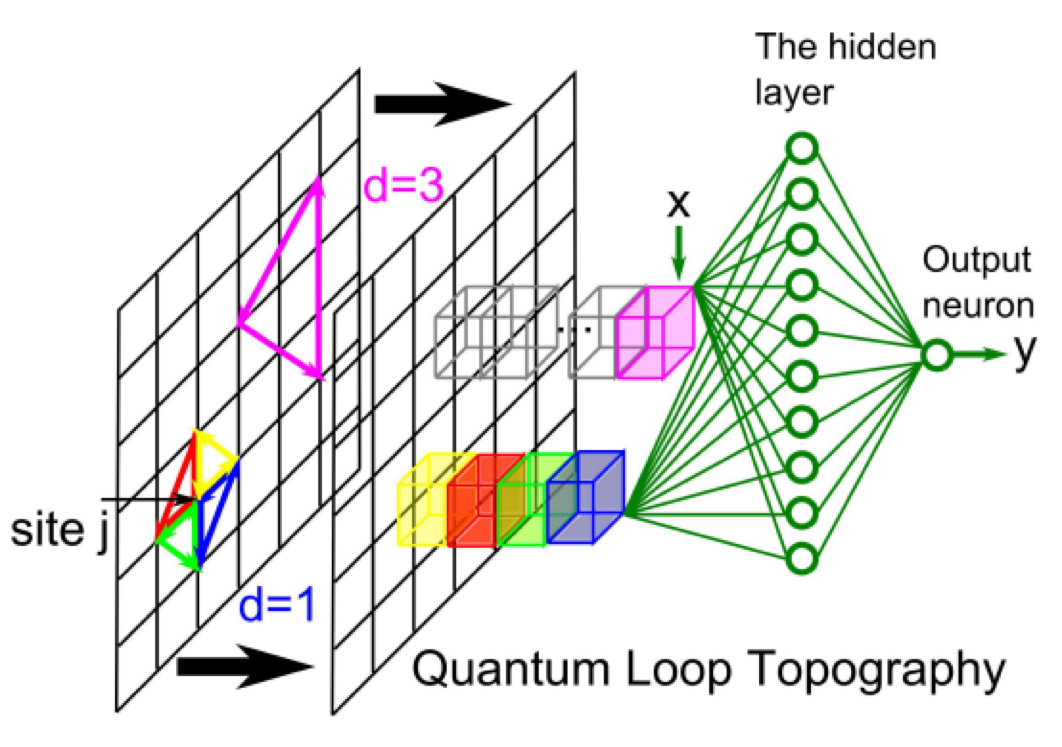
\includegraphics[width=.5\textwidth]{qlt.png}
    \caption{Caption}
    \label{fig:qlt}
\end{figure}
[6 ML architecture and preprocessing -- Trey FIG \ref{fig:qlt}]
\\
\\
\\
\\
\\
\\
\\
\\
\\
\\
\\


[7 SDW model action and what is known -- Carsten]
\\
\\
\\
\\
\\
\\
\\
\\
\\
\\

[8 2pt classification for ordered phase -- Sam/Trey. FIG \ref{fig:2ptsdw}]
\\
\\
\\
\\
\\
\\
\\
\\
 \begin{figure} [t]
    \centering
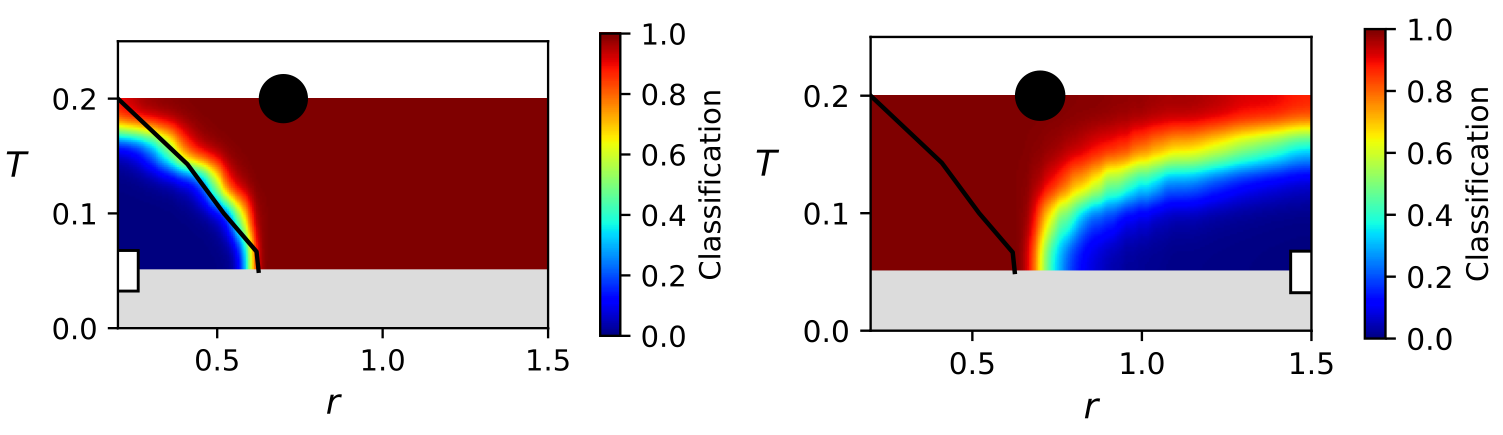
\includegraphics[width=.45\textwidth]{2PT-SDW.png}
    \caption{Caption}
    \label{fig:2ptsdw}
\end{figure}

[9 2PT classification for NFL-FL and 3PT classification --Sam/Trey]
FIG \ref{fig:2ptsdw}, FIG \ref{fig:pds}
\\
\\
\\
\\
\\
\\
\\
\\




[10 Nematic action and what is known -- Sam/Trey]
\\
\\
\\
\\
\\
\\
\\
\\
\\

\begin{figure} [t]
    \centering
    \subfigure[]{
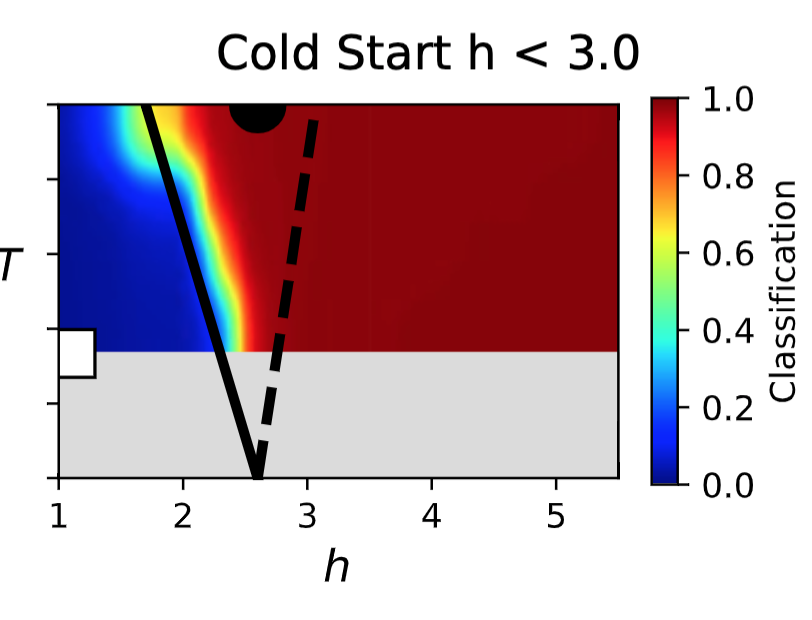
\includegraphics[width=.22\textwidth]{2PT-nematic-order.png}}
    \subfigure[]{
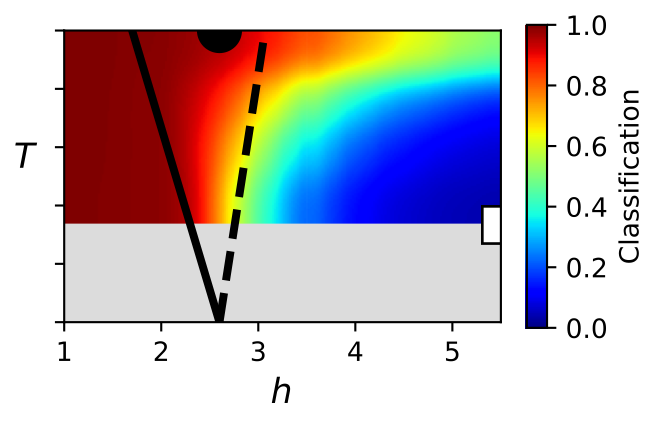
\includegraphics[width=.22\textwidth]{2PT-nematic.png}}

    \caption{Caption}
    \label{fig:2ptnem}
\end{figure}

[11 2PT classification for ordered phase -- Sam/Trey]
FIG \ref{fig:2ptnem}
\\
\\
\\
\\
\\
\\
\\
\\
\\
\\


[12 2PT classification for NFL-FL and 3pt classification --Sam/Trey]
FIG \ref{fig:2ptnem}, FIG \ref{fig:pds}.
\\
\\
\\
\\
\\
\\
\\
\\
\\

[13 Summary --EK]

[14 Implications and Outlook --EK]



{\it Acknowledgements.--} 
We acknowledge useful discussions with XXX. SL and E-AK acknowledge the support from the U.S. Department of Energy, Office of Basic Energy Sciences, Division of Materials Science and Engineering under Award DE-SC0018946.
The Cologne group acknowledges partial support from the Deutsche Forschungsgemeinschaft (DFG, German Research Foundation) -- Projektnummer 277101999 -- TRR 183 (project B01).
The numerical simulations were performed on the JUWELS cluster at FZ J\"ulich and the CHEOPS cluster at RRZK Cologne.


%\bibliographystyle{apsrev4-1}
%\bibliography{refs,t+X-NSF}
\appendix



\end{document}
